% !TeX root = RJwrapper.tex
\title{ggplot2 compatible Quantile-quantile plots in R}
\author{by Alexandre Almeida, Adam Loy, Heike Hofmann}

\maketitle

\abstract{%
An abstract of less than 150 words.
}

\newcommand{\hh}[1]{{\textcolor{orange}{#1}}}
\newcommand{\al}[1]{{\textcolor{violet}{#1}}}
\newcommand{\alex}[1]{{\textcolor{green}{#1}}}

\subsection{TODO:}\label{todo}

\begin{itemize}
\tightlist
\item
  Abstract
\item
  Give examples

  \begin{itemize}
  \tightlist
  \item
    Heike: BRFSS example
  \end{itemize}
\item
  Conclusion
\end{itemize}

\subsection{Background}\label{background}

\label{sec:introduction}

Univariate distributional assessment is a common thread throughout
statistical analyses during both the exploratory and confirmatory
stages. When we begin exploring a new data set we often consider the
distribution of individual variables before moving on to explore
multivariate relationships. After a model has been fit to a data set, we
must assess whether the distributional assumptions made are reasonable,
and if they are not, then we must understand the impact this has on the
conclusions of the model. Graphics provide arguably the most common way
to carry out these univariate assessments. While there are many plots
that can be used for distribution exploration and assessment, a
quantile-quantile (Q-Q) plot \citep{Wilk1968-ii} is one of the most
common plots used.

Q-Q plots compare two distributions by matching a commmon set of
quantiles. To compare a sample, \(y_1, y_2, \ldots, y_n\) to a
theoretical distribution, a Q-Q plot is simply a scatterplot of the
sample quantiles, \(y_{(i)}\), against the corresponding quantiles from
the theoretical distribution, \(F^{-1}\left( F_n(y_i) \right)\). If the
empirical distribution is consistent with the theoretical distribution,
then the Q-Q plot will be linear. For example, Figure \ref{fig:ex-qq1}
shows two Q-Q plots: the left plot compares a sample drawn from the
lognormal distribution to the lognormal distribution, while the right
plot compares a sample drawn from the lognormal distribution to the
normal distribution. As expected, the lognormal Q-Q plot is
approximately linear as the data and model are in agreement, while the
normal Q-Q plot is curved, indicating disagreement between the data and
the model.

\begin{Schunk}
\begin{figure}

{\centering 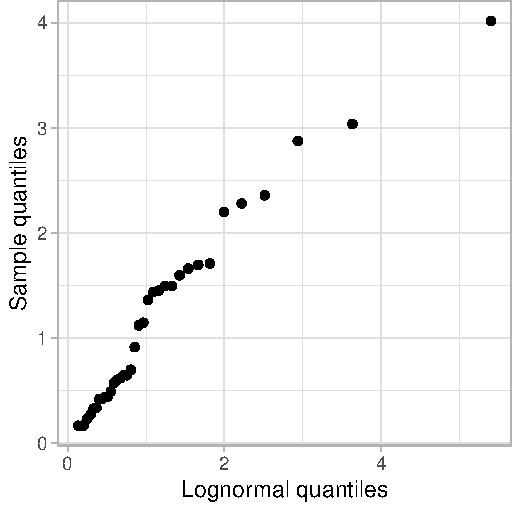
\includegraphics[width=.4\linewidth]{qqplotr_files/figure-latex/ex-qq1-1} 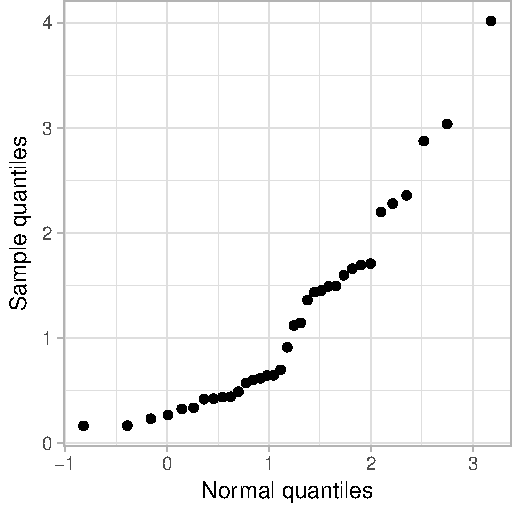
\includegraphics[width=.4\linewidth]{qqplotr_files/figure-latex/ex-qq1-2} 

}

\caption[The left plot compares a sample drawn from the lognormal distribution to the lognormal distribution, while the right plot compares a sample drawn from the lognormal distribution to the normal distribution]{The left plot compares a sample drawn from the lognormal distribution to the lognormal distribution, while the right plot compares a sample drawn from the lognormal distribution to the normal distribution. The curvature in the normal Q-Q plot highlights the disagreement betweeen the data and the model.}\label{fig:ex-qq1}
\end{figure}
\end{Schunk}

Additional graphical elements are often added to Q-Q plots in order to
aid in distributional assessment. A reference line is often added to a
Q-Q plot to assist the detection of departures from normality. This line
is often drawn by connecting the first and third quartiles. Pointwise or
simultaneous confidence bands are also frequently built around the
reference line to display the expected degree of sampling error for the
proposed model, so that minor deviations from the reference line are not
over-interpreted. Figure \ref{fig:ex-qq2} adds such reference lines and
95\% pointwise confidence bands to the Q-Q plots in Figure
\ref{fig:ex-qq1}.

\begin{Schunk}
\begin{figure}

{\centering 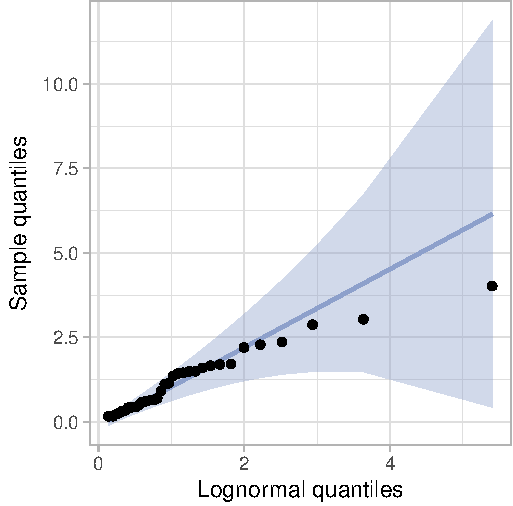
\includegraphics[width=.4\linewidth]{qqplotr_files/figure-latex/ex-qq2-1} 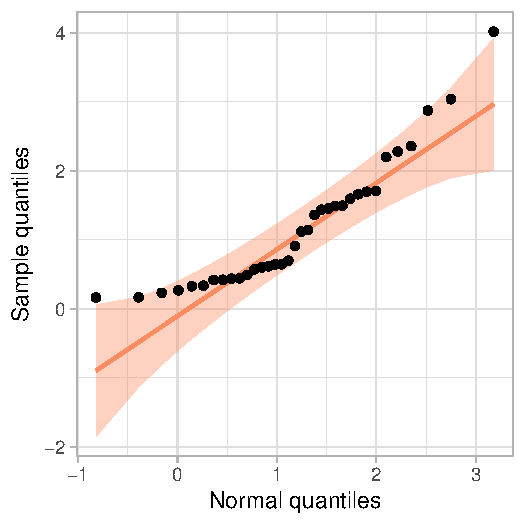
\includegraphics[width=.4\linewidth]{qqplotr_files/figure-latex/ex-qq2-2} 

}

\caption[Adding reference lines and $95\%$ pointwise confidence bands to the Q-Q plots in Figure 1]{Adding reference lines and $95\%$ pointwise confidence bands to the Q-Q plots in Figure 1.}\label{fig:ex-qq2}
\end{figure}
\end{Schunk}

Different orientations of Q-Q plots have also been proposed, most
notably the de-trended Q-Q plot. To detrend a Q-Q plot, the \(y\)-axis
is changed to show the difference between the observed quantile and the
reference line. Consequently, the line representing the agreement with
the theoretical distribution is the \(x\)-axis. \citet{Loy2016-fg} find
that detrended Q-Q plots are more powerful than other designs,
\al{so long as $x$- and $y$-axes to show the same range. Adjusting the aspect ratio in this way ensures that distances in the $x$- and $y$-directions are on the same scale. This Q-Q plot design is called an *adjusted-detrended Q-Q plot*.  If the range of the axes are not adjusted, then this results an ordinary detrended Q-Q plot, which which was found to have lower power than the standard Q-Q plot in some situations \citep{Loy2016-fg}.}
Figure \ref{fig:ex-detrend} displays the normal Q-Q plot from Figure
\ref{fig:ex-qq2} along with its adjusted detrended version.

\begin{Schunk}
\begin{figure}

{\centering 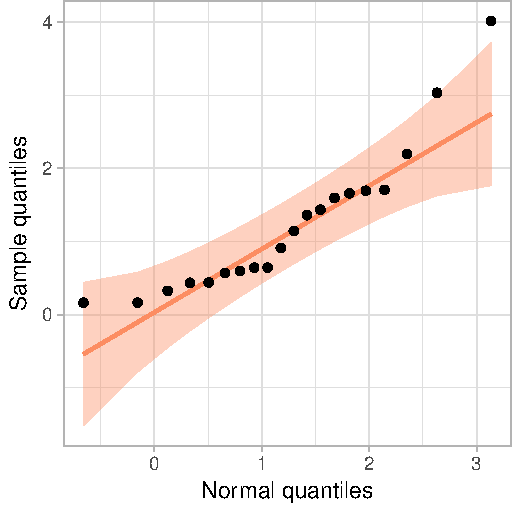
\includegraphics[width=.4\linewidth]{qqplotr_files/figure-latex/ex-detrend-1} 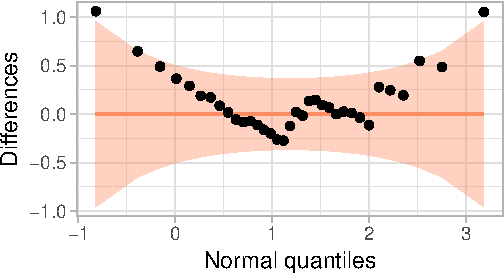
\includegraphics[width=.4\linewidth]{qqplotr_files/figure-latex/ex-detrend-2} 

}

\caption[The left plot displays a traditional normal Q-Q plot for data simulated from a lognormal distribution]{The left plot displays a traditional normal Q-Q plot for data simulated from a lognormal distribution. The right plot displays an adjusted detrended Q-Q plot of the same data, created by plotting the differences between the sample quantiles and the proposed model on the $y$-axis.}\label{fig:ex-detrend}
\end{figure}
\end{Schunk}

Various implementations of Q-Q plots exist in R. Normal Q-Q plots, where
a sample is compared to the standard normal distribution, are
implemented using \texttt{qqplot} and \texttt{qqline} in \pkg{base}
graphics \citep{R}. \pkg{lattice} provides a general framework for Q-Q
plots in the \texttt{qqmath} function, allowing one to compare a sample
to any theoretical distribution by specifying the appropriate quantile
function \citep{lattice}. \texttt{qqPlot} in the \pkg{car} package also
allows for the assessment of non-normal distributions and adds pointwise
confidence bands via normal theory or the parametric bootstrap
\citep{car}. \pkg{ggplot2} provides \texttt{geom\_qq} and
\texttt{geom\_qq\_line}, enabling the creation of Q-Q plots with a
reference line, much like those created using \texttt{qqmath}
\citep{ggplot2}. None of these general use packages allow for easy
construction of de-trended Q-Q plots.

\pkg{qqplotr} extends \pkg{ggplot2} to provide a complete implementation
of Q-Q plots. The package allows for quick construction of all Q-Q plot
designs without sacrificing the flexibility of the \pkg{ggplot2}
framework. In the remainder of this paper, we will introduce the
plotting framework provided by \pkg{qqplotr} and provide multiple
examples of how it can be used.

\subsection{\texorpdfstring{Implementing Q-Q plots in the \pkg{ggplot2}
framework}{Implementing Q-Q plots in the  framework}}\label{implementing-q-q-plots-in-the-framework}

With \pkg{qqplotr} we extend some of the original \pkg{ggplot2} Q-Q plot
functionatilites by permitting the drawing of Q-Q points, lines, and
confidence bands. Our approach provides a \pkg{ggplot2} layering
mechanism so that for each one of those plot elements we implemented a
\pkg{ggplot2} ``stat'' (statistical transformation). In addition, we
also implemented a \pkg{ggplot2} ``geom'' (geometrical object)
specifically for the confidence bands. That geom permits a simpler way
of handling graphical parameters, which will become clearer in the
\nameref{sec:examples} section.

The Q-Q plot functions are divided into three statistical
transformations. Below, we describe each one of those functions and also
give an overview of its parameters.

\subsubsection{\texorpdfstring{\texttt{stat\_qq\_point}}{stat\_qq\_point}}\label{stat_qq_point}

This is a modified version of \texttt{stat\_qq}/\texttt{geom\_qq} from
\pkg{ggplot2} that plots the sample quantiles versus the theoretical
quantiles (as in Figure \ref{fig:ex-qq1}). The novelty of this
implementation is an option to detrend the plotted points (see
\nameref{sec:introduction}). Note that all other implemented functions
in the \pkg{qqplotr} package also allow for this option. Below we
present a complete call to \texttt{stat\_qq\_point} and highlight its
default parameters values:

\begin{Schunk}
\begin{Sinput}
stat_qq_point(
  data = NULL,
  mapping = NULL,
  geom = "point",
  position = "identity",
  na.rm = TRUE,
  show.legend = NA,
  inherit.aes = TRUE,
  distribution = "norm",
  dparams = list(),
  detrend = FALSE,
  qtype = 7,
  qprobs = c(0.25, 0.75),
  ...
  )
\end{Sinput}
\end{Schunk}

\begin{itemize}
\item
  Parameters such as \texttt{data}, \texttt{mapping}, \texttt{geom},
  \texttt{position}, \texttt{na.rm}, \texttt{show.legend}, and
  \texttt{inherit.aes} are specific for \pkg{ggplot2} implementations.
\item
  \texttt{distribution} is a character string that sets the theoretical
  probability distribution. Here, we followed the nomenclature from the
  \pkg{stats} package. You must not provide the full distribution
  function name (e.g., \texttt{"dnorm"}). Instead, just provide its
  suffix (e.g., \texttt{"norm"}). If you wish to provide a custom
  distribution (as we will do in Section \ref{sec:user-dists}), you may
  do so by first creating the density (PDF), distribution (CDF),
  quantile, and random functions (also by following \pkg{stats} package
  nomenclature, i.e., for \texttt{"custom"}, you must provide the
  \texttt{dcustom}, \texttt{pcustom}, \texttt{qcustom}, and
  \texttt{rcustom} functions).
\item
  \texttt{dparams} is a named list to be provided alongside with the
  previously chosen \texttt{distribution}. By default, MLEs are used for
  the distributional parameters. By manually providing any of the
  distributional parameters, the MLE is automatically turned off. Please
  note that MLEs are currently only supported for distributions
  available in the \pkg{stats} package; if a custom distribution is used
  in \texttt{distribution} \emph{all} of its parameters have to be
  provided in \texttt{dparams}.
\item
  \texttt{detrend} is a boolean that controls whether the points should
  be detrended (as shown in Figure \ref{fig:ex-detrend}). More on that
  in Section \ref{sec:detrending}.
\item
  \texttt{qtype} and \texttt{qprobs} are only used when
  \texttt{detrend\ =\ TRUE}. These parameters are passed on to the
  \texttt{type} and \texttt{probs} parameters of \texttt{quantile}
  function from the \pkg{stats} package. The \texttt{quantile} function
  is used to define the quantiles where the reference line (i.e., the
  proposed model) shall intercept.
\end{itemize}

\subsubsection{\texorpdfstring{\texttt{stat\_qq\_line}}{stat\_qq\_line}}\label{stat_qq_line}

This statistical transformation draws a reference line based on the
sample data quantiles. Note that the \texttt{stat\_qq\_line} call below
does not present any additional parameters when compared to
\texttt{stat\_qq\_point}.

\begin{Schunk}
\begin{Sinput}
stat_qq_line(
  data = NULL,
  mapping = NULL,
  geom = "path",
  position = "identity",
  na.rm = TRUE,
  show.legend = NA,
  inherit.aes = TRUE,
  distribution = "norm",
  dparams = list(),
  detrend = FALSE,
  qtype = 7,
  qprobs = c(0.25, 0.75),
  ...
  )
\end{Sinput}
\end{Schunk}

\hh{By default this line is drawn through two points, corresponding to the 25 and 75 percentile of the distributions on $x$ (theoretical distribution) and $y$ (empirical distribution).  While we are using MLE to identify the exact distribution to compare against, these estimates are only used in determining the $x$-coordinates of these points. For the $y$ coordinates 1st and 3rd quartile are used by default for a more robust estimation. The difference between observed and theoretical distribution therefore presents itself in the difference between the Q-Q line and the identity line. Using robust estimates for the Q-Q line is of particular advantage for small samples \citep{Loy2016-fg}.}

\subsubsection{\texorpdfstring{\texttt{stat\_qq\_band}}{stat\_qq\_band}}\label{stat_qq_band}

Draws confidence bands around the reference line using one of three
methods: a normal approximation, the parametric bootstrap, or the
tail-sensitive procedure. Below, we present the call to
\texttt{stat\_qq\_band} and describe its specific parameters:

\begin{Schunk}
\begin{Sinput}
stat_qq_band(
  data = NULL,
  mapping = NULL,
  geom = "qq_band",
  position = "identity",
  show.legend = NA,
  inherit.aes = TRUE,
  na.rm = TRUE,
  distribution = "norm",
  dparams = list(),
  detrend = FALSE,
  qtype = 7,
  qprobs = c(0.25, 0.75),
  bandType = "normal",
  B = 1000,
  conf = 0.95,
  mu = NULL,
  sigma = NULL,
  ...
  )
\end{Sinput}
\end{Schunk}

\begin{itemize}
\item
  \texttt{bandType} is a character string that controls the method to be
  used when constructing the confidence bands:

  \begin{itemize}
  \tightlist
  \item
    \textbf{Normal:} Specifying \texttt{bandType\ =\ "normal"}
    constructs pointwise confidence bands based on the normal
    approximation to the distribution of the order statistics. For
    example, an approximate 95\% confidence interval for the \(i\)th
    order statistic is
    \(\widehat{X}_{(i)}~\pm~\Phi^{-1}(.975)~\cdot~SE(X_{(i)})\), where
    \(\widehat{X}_{(i)}\) denotes the value along the fitted line,
    \(\Phi^{-1}(\cdot)\) denotes the quantile function for the standard
    normal distribution, and \(SE(X_{(i)})\) is the standard error of
    the \(i\)th order statistic.
  \item
    \textbf{Bootstrap:} Specifying \texttt{bandType\ =\ "bs"} constructs
    pointwise confidence bands using percentile confidence intervals
    from the parametric bootstrap.
  \item
    \textbf{Tail-sensitive:} Specifying \texttt{bandType\ =\ "ts"}
    constructs the simulation-based tail-sensitive simultaneous
    confidence bands proposed by \citet{Aldor-Noiman2013-xw}.
  \end{itemize}
\item
  \texttt{B} is an integer that represents the number of bootstrap
  replicates (if \texttt{bandType\ =\ "bs"}) or the number of simulated
  samples (if \texttt{bandType\ =\ "ts"}).
\item
  \texttt{conf} is a numerical variable that controls the confidence
  level of the bands, which must be a value between 0 and 1.
\item
  \texttt{mu} and \texttt{sigma} are only used when
  \texttt{bandType\ =\ "ts"}. They represent the center and scale
  distributional parameters, respectively, which are used used to
  construct the simulated tail-sensitive confidence bands. If any of the
  parameters is provided with \texttt{NULL}, then both the center and
  scale parameters will be estimated using robust estimates via the
  \texttt{robustbase} package.
\end{itemize}

\subsubsection{\texorpdfstring{facetting and
\texttt{qqplotr}}{facetting and qqplotr}}\label{facetting-and-qqplotr}

\hh{placeholder for now: discuss groups and facets }

\FloatBarrier

\subsection{Examples}\label{examples}

\label{sec:examples}

In this section, we demonstrate the capabilities of the \pkg{qqplotr}
package. We start by loading the package:

\begin{Schunk}
\begin{Sinput}
library(qqplotr)
\end{Sinput}
\end{Schunk}

\subsubsection{\texorpdfstring{Constructing Q-Q plots with
\texttt{qqplotr}}{Constructing Q-Q plots with qqplotr}}\label{constructing-q-q-plots-with-qqplotr}

\alex{Placeholder subsection name}

To give a brief introduction on how to use \pkg{qqplotr} and its
functions, let us use as example the \texttt{urine} dataset of the
\pkg{boot} package. This small dataset presents 79 urine specimens that
were analyzed in order to determine if certain physical characteristics
of the urine (e.g.~pH, urea concentration) might be related to the
formation of calcium oxalate crystals. Here, we will focus on
distributional assessment of the urine samples pH measurements.

\alex{The idea of this subsection is to briefly exemplify the usage of the implemented functions of qqplotr, while also showcasing the three methods for constructing the confidence bands. Hence, I've included this dataset because of the distinct conclusions that can be made based on the visual inference of the pH measurement QQ-plots when using the three confidence bands methods, which justifies their implementation.}

\alex{TODO: Still need to display essential code chunks in the paper, add a Figure with the 3 band types side-by-side, and discuss all the Figures.}

\begin{Schunk}
\begin{figure}

{\centering \includegraphics[width=0.45\textwidth]{qqplotr_files/figure-latex/tooth-qq-1} 

}

\caption[Placeholder caption]{Placeholder caption.}\label{fig:tooth-qq}
\end{figure}
\end{Schunk}

\subsubsection{BRFSS example}\label{brfss-example}

The Center for Disease Control and Prevention runs an annual telephone
survey, the Behavioral Risk Factor Surveillance System (BRFSS), to keep
track of the US populations' `health-related risk behaviors, chronic
health conditions, and use of preventive services'.

Close to half a million interviews are conducted each year. Here, we are
focussing on the 2012 responses for Iowa. 7166 responses were gathered
across 359 questions and derived variables. Among these, are
participants' heights and weights, which we are going to assess in more
detail.

Figure \ref{fig:heights} shows two Q-Q plots side by side. For each of
the plots, a sample of 200 men and 200 women is drawn from the overall
number of responses. On the left hand side, individuals' heights are
plotted in a Q-Q plot comparing raw heights to a normal distribution. We
see that the distributions for both men and women (colour) is showing
horizontal steps: this indicates that the distributional assessement is
heavily dominated by the discreteness in the data, as most survey
participants responded to the question of their height only up to the
closest inch. On the right hand side of Figure \ref{fig:heights}, we use
jittering; this means that we add a random number generated from a
random uniform distribution on \(\pm 0.5\) inch to the reported height,
as shown in the code below:

By using jittering we diminish the effect that discreteness has on the
distribution and brings the observed distribution much closer to a
normal distribution. Note that separate normal distributions were fitted
for each gender. Not surprisingly, the resulting distributions have
different means (women are on average 6 inch shorter than men in this
dataset). Interestingly, the slope of the two genders is similar,
indicating that the same scale parameter fits both genders'
distributions (the standard deviation of height in the data set is 2.97
inch for men and 2.91 inch for women, see Table \ref{tab:heights}). The
dark line between the two groups is the identity line -- representing
the theoretical distribution each of these groups are compared to. This
distribution is based on parameters estimated from the whole population
(see Table \ref{tab:heights} for numbers) . While the mean is about half
way between the gender means, we see from the higher slope of the line
that in comparison to each group, the standard deviation of the height
based on the whole population is larger.

\begin{table}

\caption{\label{tab:heights-table}Summary of Iowa's residents' heights and weights with corresponding standard deviations by gender and for the total population.\label{tab:heights}}
\centering
\begin{tabular}[t]{lrrrr}
\toprule
SEX & mean height (in inch) & sd (in inch) & mean log weight (in kg) & sd (in kg)\\
\midrule
Male & 70.55 & 2.97 & 9.10 & 0.20\\
Female & 64.51 & 2.91 & 8.89 & 0.23\\
Total & 66.99 & 4.18 & 8.98 & 0.24\\
\bottomrule
\end{tabular}
\end{table}

\begin{Schunk}
\begin{figure}

{\centering 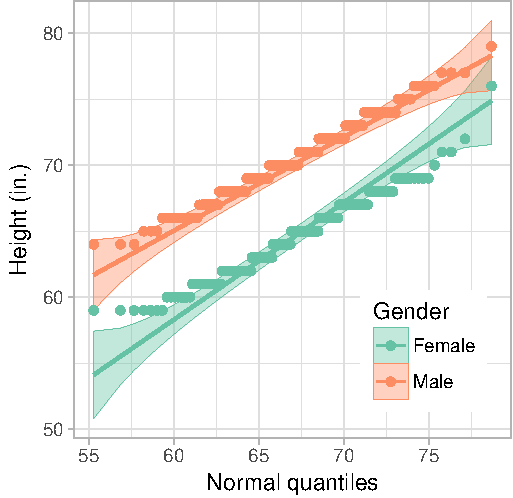
\includegraphics[width=\textwidth]{qqplotr_files/figure-latex/heights-1} 

}

\caption[Sample (200 men and 200 women) of raw heights (left) and jittered heights (right)]{Sample (200 men and 200 women) of raw heights (left) and jittered heights (right). The distribution on the left is dominated by the discreteness of the data. On the right we see that except for some outliers an assumption of normality for people's height is not completely absurd.}\label{fig:heights}
\end{figure}
\end{Schunk}

Unlike respondents' heights, their weights do not seem to be normally
distributed. Figure \ref{fig:weights} shows again two Q-Q plots. The Q-Q
plot on the left uses raw weights and compares to a normal distribution.
From the deviation in the extremes we see that tails of the observed
distribution are heavier than expected under a normal distribution. On
the right, weights are log-transformed. We see that a normal
distribution for each of the genders shows --with the exceptions of a
few extreme outliers-- a reasonable fit.

\begin{Schunk}
\begin{figure}

{\centering 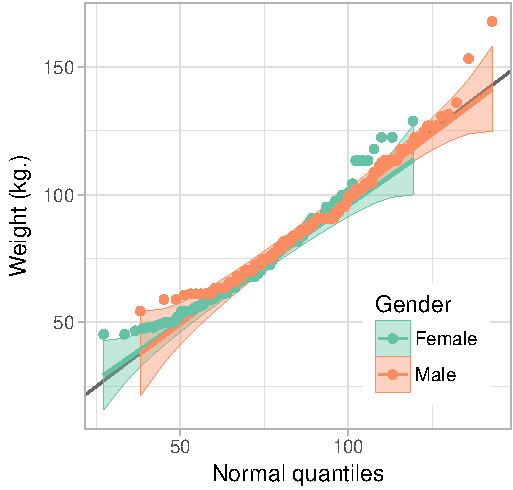
\includegraphics[width=\textwidth]{qqplotr_files/figure-latex/weights-1} 

}

\caption[Sample (200 men and 200 women) of weights]{Sample (200 men and 200 women) of weights. Unlike people's height, weight seems to be heavily right skewed with some additional outliers on the extreme left (left plot). On the right, weight was log-transfomed before its distribution is compared to a theoretical normal. }\label{fig:weights}
\end{figure}
\end{Schunk}

Instead of transforming the observed values, we can change the
theoretical distribution against which we compare. Figure
\ref{fig:weights-log} shows two Q-Q plots, one for each of the genders.
A log-normal distribution is chosen as the theoretical distribution. By
default, for each of the groups ML estimates are used:

\begin{Schunk}
\begin{Sinput}
p6 <- sample_ia %>% 
  ggplot(aes(sample = WTKG3 / 100, colour = Gender, fill = Gender)) +
  geom_abline(colour="grey60") +
  stat_qq_band(distribution = "lnorm", alpha = 0.3) +
  stat_qq_line(distribution = "lnorm") +
  stat_qq_point(distribution = "lnorm") +
  scale_fill_brewer(palette = "Set1") +
  scale_colour_brewer(palette = "Set1") +
  customization + facet_grid(.~Gender)
\end{Sinput}
\begin{figure}

{\centering 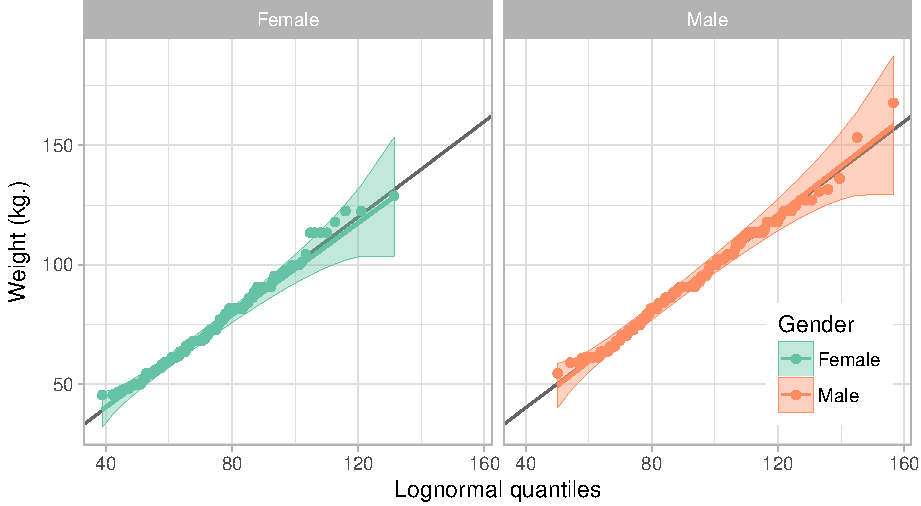
\includegraphics[width=.9\textwidth]{qqplotr_files/figure-latex/weights-log-1} 

}

\caption[Sample (200 men and 200 women) of weights, the theoretical distribution  is changed to a log normal]{Sample (200 men and 200 women) of weights, the theoretical distribution  is changed to a log normal. Shift and scale parameters are estimated separately for each of the genders before comparing distributions to a log-normal.}\label{fig:weights-log}
\end{figure}
\end{Schunk}

\subsubsection{Using user-provided
distributions}\label{using-user-provided-distributions}

\label{sec:user-dists}

\al{Question: Should we move these sections above the BRFSS section, since they are a bit more straightforward?}

Using the capabilities of \pkg{qqplotr} with the distributions
implemented in the \pkg{stats} package is relatively straightfoward,
since the implementation allows you to specify the suffix
(i.e.~distribution and or abbreviation) via the \texttt{distribution}
argument and the parameter estimates via \texttt{dparams} argument.
However, there are times when the distributions in \pkg{stats} are not
sufficient for the demands of the analysis. For example, there is no
left-skewed distribution listed. User-coded distributions or
distributions from other packages can be used with \pkg{qqplotr} as long
as the distributions are defined following the conventions laid out in
the \pkg{stats} package. Specfically, for some distribution there must
be density/mass (\texttt{d} prefix), CDF (\texttt{p} prefix), quantile
(\texttt{q} prefix), and simulation (\texttt{r} prefix) functions. In
this section we illustrate the use of the smallest extreme value
distribution (SEV).

To qualify for the Olympics in the men's long jump in 2012, athletes had
to either meet/exceed the 8.1 meter standard or place in the top twelve.
During the qualification events, each athlete was able to jump three
times, and their best (i.e.~longest) jump is treated as the result.
Figure \ref{fig:jump-density} shows a density plot of the results, which
are cleaerly left skewed.

\begin{Schunk}
\begin{figure}

{\centering 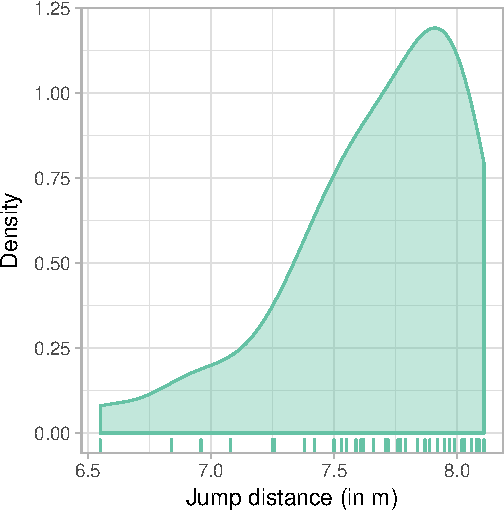
\includegraphics[width=0.45\textwidth]{qqplotr_files/figure-latex/jump-density-1} 

}

\caption[Density plot of the 2012 men's long jump qualifying round]{Density plot of the 2012 men's long jump qualifying round. The distances are clearly left skewed.}\label{fig:jump-density}
\end{figure}
\end{Schunk}

In order to model the jump distances we must first define a left-skewed
distribution. Below, we define the suite of distributional functions
necessary to utilize the SEV distribution.

\begin{Schunk}
\begin{Sinput}
# CDF
psev <- function(q, mu = 0, sigma = 1) {
    z <- (q - mu) / sigma
    1 - exp(-exp(z))
}

# PDF
dsev <- function(x, mu = 0, sigma = 1) {
  z <- (x - mu) / sigma
  (1 / sigma) * exp(z - exp(z))
}

# Quantile function
qsev <- function(p, mu = 0, sigma = 1) {
  mu + log(-log(1 - p)) * sigma
}

# Simulation function
rsev <- function(n, mu = 0, sigma = 1) {
  qsev(runif(n), mu, sigma)
}
\end{Sinput}
\end{Schunk}

With the \texttt{*sev} distribution functions in hand, we can create a
Q-Q plot to assess the appropriateness of the SEV model (Figure
\ref{fig:sev-qq}). The Q-Q plot show that the distances do not
substantially deviate from the SEV model, so we have found an adequate
representation of the distances.

\begin{Schunk}
\begin{Sinput}
ggplot(longjump, aes(sample = distance)) +
  stat_qq_band(distribution = "sev", dparams = list(mu = 0, sigma = 1), alpha = 0.3) +
  stat_qq_line(distribution = "sev", dparams = list(mu = 0, sigma = 1)) +
  stat_qq_point(distribution = "sev", dparams = list(mu = 0, sigma = 1)) +
  xlab("Theoretical quantiles") +
  ylab("Jump distance (in m)") +
  theme_bw()
\end{Sinput}
\begin{figure}

{\centering 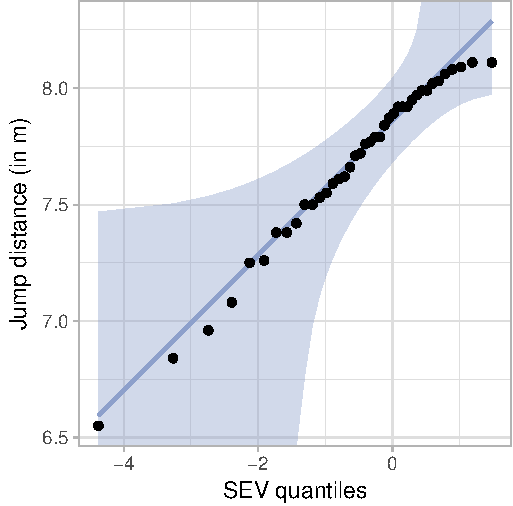
\includegraphics[width=0.45\textwidth]{qqplotr_files/figure-latex/sev-qq-1} 

}

\caption[Q-Q plot comparing the long jump distances to the standard SEV distribution]{Q-Q plot comparing the long jump distances to the standard SEV distribution. The SEV distribution appears to adequately model the distances.}\label{fig:sev-qq}
\end{figure}
\end{Schunk}

\subsubsection{Detrending Q-Q plots}\label{detrending-q-q-plots}

\label{sec:detrending}

\al{AL: It seems natural to have a subsection here, even if we continue the example, to allow people to skim the paper and find the topic they are most interested in. I tried to eliminate the techinical discussion of the plot since it is in the background section, instead describing the code. What do you think?}

To illustrate how to construct an adjusted detrended Q-Q plot using
\pkg{qqplotr}, consider detrending the Q-Q plot in Figure
\ref{fig:sev-qq}. To obtain a detrended version of Figure
\ref{fig:sev-qq}, we must add the argument \texttt{detrend\ =\ TRUE} to
\texttt{stat\_qq\_point}, \texttt{stat\_qq\_line}, and
\texttt{stat\_qq\_band}. To adjust the aspect ratio to ensure that
vertical and horizontal distances are on the same scale we further add
\texttt{theme(aspect.ratio\ =\ 1)}.

\begin{Schunk}
\begin{figure}

{\centering 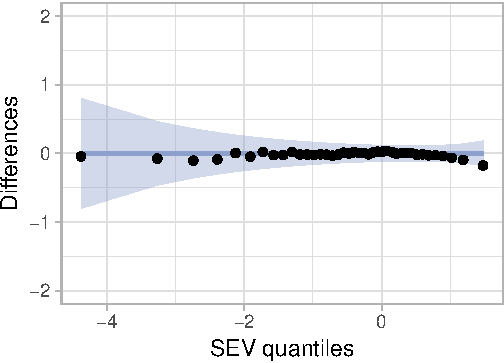
\includegraphics[width=0.45\textwidth]{qqplotr_files/figure-latex/detrend-sev-1} 

}

\caption[An adjusted detrended Q-Q plot assessing the appropriateness of the SEV distribution for the long jump data]{An adjusted detrended Q-Q plot assessing the appropriateness of the SEV distribution for the long jump data.}\label{fig:detrend-sev}
\end{figure}
\end{Schunk}

\begin{Schunk}
\begin{Sinput}
ggplot(longjump, aes(sample = distance)) +
  stat_qq_band(distribution = "sev", alpha = 0.3, detrend = TRUE, dparams = c(mu = 0, sigma = 1)) +
  stat_qq_line(distribution = "sev", detrend = TRUE, dparams = c(mu = 0, sigma = 1)) +
  stat_qq_point(distribution = "sev", detrend = TRUE, dparams = c(mu = 0, sigma = 1)) +
  xlab("Theoretical quantiles") +
  ylab("Differences") +
  theme_bw() +
  theme(aspect.ratio = 1)
\end{Sinput}
\end{Schunk}

\subsubsection{Q-Q plots with robust
estimators}\label{q-q-plots-with-robust-estimators}

\al{What do we really want to highlight with robust estimators? I am ready to write this section, but am unsure what to highlight: the different lines? the dparams?}

\begin{Schunk}
\begin{Sinput}
set.seed(798534)
t_data <- rt(20, df = 2)
norm_data <- rnorm(20)
chisq1 <- rchisq(20, df = 1)
\end{Sinput}
\end{Schunk}

\subsection{Discussion}\label{discussion}

This paper presents the \pkg{qqplotr} package, an extension of
\pkg{ggplot2} that implements Q-Q plots in both the standard and
de-trended orientations, reference lines for Q-Q plots, and confidence
bands for Q-Q plots. The examples illustrate how to create Q-Q plots for
non-standard distributions found outside of the \pkg{stats}, de-trend
Q-Q plots, and create Q-Q plots when data are grouped. Further, in the
BRFSS example, we illustrated how jittering can be used in Q-Q plots to
better compare discretized data to a continuous distribution.

Q-Q plots are member of the larger probability plotting family, and
future versions of the package will incorporate additional plots into
\pkg{qqplotr}. Specifically, two types of probability plots will be
included:

\begin{enumerate}
\def\labelenumi{\arabic{enumi}.}
\tightlist
\item
  A standardarized P-P plot is constructed for location-scale
  distributions by plotting \(F(z_{(i)})\) against \(p_i\), where
  \(z_{(i)}\) denotes the ordered and standardized observations and
  \(p_i\) is denotes the plotting position \citep{Gan1991-yk}. As
  \citet{Gan1991-yk} point out, the probability plotting positions are
  equally spaced on the \(x\)-x axis, whereas points on the \(x\)-axis
  of a Q-Q plot are more concentrated in the higher-density regions of
  the reference distribution. This leads to Q-Q plots being more
  sensitive to discrepencies in the tail of the distribution and
  standardized P-P plots being more sensitive to discrepencies in the
  middle of the proposed distribution.
\item
  In engineering applications, probability plots refer to a linearized
  plot of \(F(x_i)\) against \(x_i\). This linearizing transformation of
  the hypothesized CDF is found by first finding a transformations that
  linearize the quantile function---i.e.~linearizing the plot of
  \(F^{-1}(p)\) vs \(x_p\)---and then mapping \(F^{-1}(p)\) back to the
  probability scale \citep[cf.][Chapter 6]{Meeker1998}.
\end{enumerate}

It is important to note that all of the probability plotting methods
discussed----Q-Q plots, standardized P-P plots, and probability
plots---are invariant to linear transformations. Consequently, each type
of plot will exhibit a linear relationship between the sample and
hypothesized distribution for location-scale families, even if the
location and/or scale parameters in the sample differ from the
hypothesized distribution. This is not the case with unstandardized P-P
plots \citep{Wilk1968-ii}, so they will not be included in
\pkg{qqplotr}.

\bibliography{RJreferences}

\subsection{Acknowledgements}\label{acknowledgements}

This work was partially funded by Google Summer of Code 2017.

\address{%
Alexandre Almeida\\
University of Campinas\\
Institute of Computing\\ Campinas, Brazil 13083-852\\
}
\href{mailto:almeida.xan@gmail.com}{\nolinkurl{almeida.xan@gmail.com}}

\address{%
Adam Loy\\
Carleton College\\
Department of Mathematics and Statistics\\ Northfield, MN 55057\\
}
\href{mailto:aloy@carleton.edu}{\nolinkurl{aloy@carleton.edu}}

\address{%
Heike Hofmann\\
Iowa State University\\
Department of Statistics\\ Ames, IA 50011-1210\\
}
\href{mailto:hofmann@iastate.edu}{\nolinkurl{hofmann@iastate.edu}}

